Three \acrshort{hmi}s have been configured and programmed as control sources for the lolly machine. This chapter provides detail into \acrshort{hmi} development. All \acrshort{hmi}s communicate with the \acrshort{plc} through Modbus \acrshort{tcpIp}.

\section{Siemens HMI}
    A KTP600 Siemens \acrshort{hmi} is the main control source and is permanently mounted to the front of the machine. This \acrshort{hmi} serves as a setup and diagnostic tool for operators as well as an interface for machine users. With many users being children, one of the main design consideration was that user screens needed to be simplistic with a `fun' feel about it. The layout of the screens will be discussed further in Section \ref{sec:hmiScreens}. Programming the KTP600 was done using \acrfull{tia} Portal by Siemens. Appendix \HD{HMI Appendix Number} provides programming and configuration details.

        \begin{figure}[H]
            \centering
            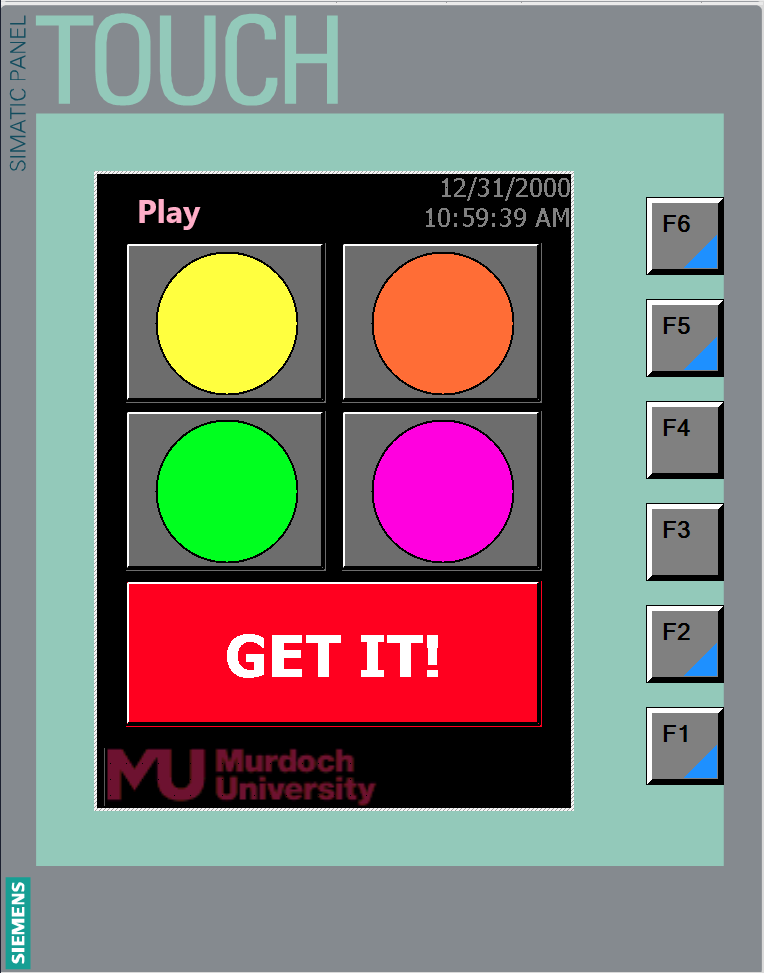
\includegraphics[width = 0.45\textwidth]{2_images/hmiPlay}
            \caption{The Siemens HMI shwoing the Play screen.}
            \label{fig:hmiPlay}
        \end{figure}    
    
    \subsection{Configuration}
        \subsubsection{Modbus Communication}
            To allow communication between the \acrshort{hmi} and the \acrshort{plc}, a connection must be added and configured within the \acrshort{hmi}. Figure \ref{fig:modbusHmiConfig} shows the configuration for the Modbus connection between the \acrshort{hmi} and \acrshort{plc}. Once a Modbus connection has been added and configured, \acrshort{hmi} tags need to be defined. \acrshort{hmi} tags are address links between the \acrshort{hmi} and the \acrshort{plc}. Objects (buttons, indicators, etc) on the \acrshort{hmi} screens are linked to tags with read and/or write access. 
            
        \begin{figure}[H]
            \centering
            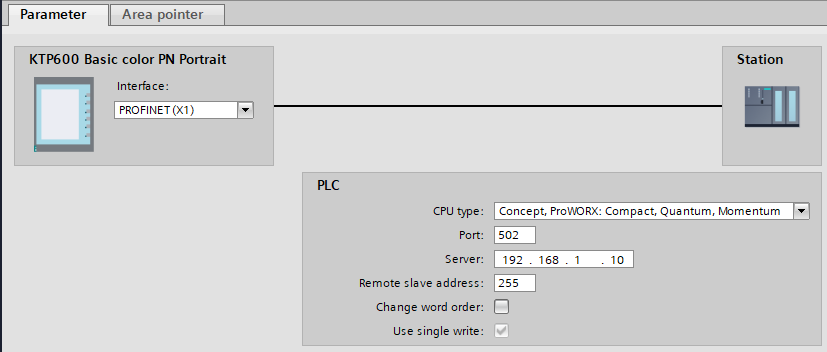
\includegraphics[width = 0.6\textwidth]{2_images/modbusHmiConfig}
            \caption{Configuration settings for a Modbus connection within the Siemens HMI.}
            \label{fig:modbusHmiConfig}
        \end{figure}        
        
        \subsubsection{Alarms}
            Two alarm Words transmitted from the \acrshort{plc} provide the \acrshort{hmi} with 21 different discrete alarms where each bit within each word is associated with a different alarm. Discrete alarms are made up of a trigger tag and a trigger bit. The tag is the alarm Word and the bit is the index of the bit within the alarm word. This is illustrated in Figure \ref{fig:hmiAlarms} below.

        \begin{figure}[H]
            \centering
            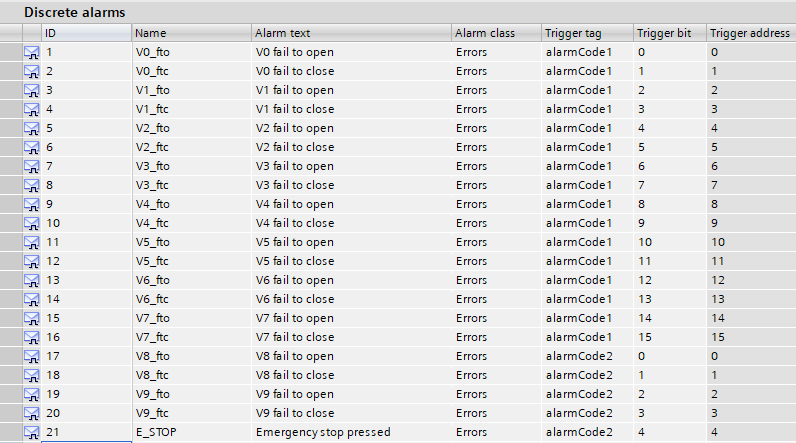
\includegraphics[width = 0.6\textwidth]{2_images/hmiAlarms}
            \caption{Alarm configuration of the Siemens HMI.}
            \label{fig:hmiAlarms}
        \end{figure}     
            
        \subsubsection{Heart Beat}
            The heartbeat from the Siemens \acrshort{hmi} is produced by a status word which Siemens refer to as the coordination area pointer. The second bit of the coordination area pointer is the `Life Bit' which is used as the heartbeat signal to the \acrshort{plc}. The coordination area pointer is linked to a Modbus address within the configuration connection.
            The startup bit and operation mode bits are not used within this project. 

        \begin{figure}[H]
            \centering
            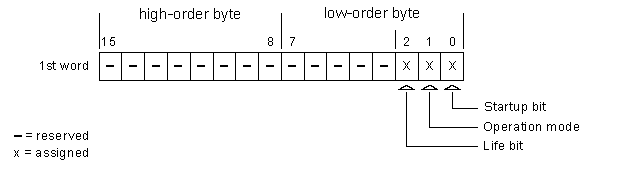
\includegraphics[width = 0.6\textwidth]{2_images/hmiCoordination}
            \caption{Coordination area pointer bit assignment}
            \label{fig:hmiAlarms}
        \end{figure} 
            

    \subsection{Screens} \label{sec:hmiScreens}
        
    
\section{LabVIEW}

    \subsection{Back Panel}

        \subsubsection{Modbus Communication}

        \subsection{Watch Dog Timer}
        
        \subsection{Data Conversion}

    \subsection{Front Panel}



\section{Raspberry-Pi/ Node-RED}
    Node-RED is a programming tool that links hardware devices, \acrshort{api}s and online services through a new method which looks similar to a flow diagram. For this project, Node-RED is hosted on a Raspberry Pi Microcontroller and is used to link WiFi enabled devices (smart phones, tablets, computers, etc) to the \acrshort{plc}.

    \subsection{Raspberry Pi}
        The Raspberry Pi used in this project has been configured as a \acrshort{wap} to allow a remote connection from WiFi enabled devices. 
    
    \subsection{Node-RED Flow}
        \subsubsection{Modbus Communication}

        \subsubsection{Watch Dog Timer}
    
    \subsection{Node-RED Dashboard}

\section{Physical Push Buttons and LED Indicators}
    Although the physical push buttons and \acrshort{led}s are not by definition a \acrshort{hmi}, they are  
    
    
